\documentclass[aps,
%prl,
twocolumn,
showpacs,
superscriptaddress,groupedaddress]{revtex4}


\usepackage{amssymb}
\usepackage{amsmath}
\usepackage{float}
\usepackage{graphicx}
\usepackage[caption=false]{subfig}
\usepackage{subfig}
\usepackage{mathrsfs}

\newcommand{\dmcomment}[1]{{\tt #1}}

\begin{document}

\title{Theory of the crossover from lasing to steady state superradiance}
\author{D. A. Tieri}
\affiliation{JILA, University of Colorado, Boulder}
\author{Minghui Xu}
\affiliation{JILA, University of Colorado, Boulder}
\author{D. Meiser}
\affiliation{Tech-X Corporation, 5621 Arapahoe Avenue,
             Boulder, Colorado 80303, USA.}
\author{J. Cooper}
\affiliation{JILA, University of Colorado, Boulder}
\author{M. J. Holland}
\affiliation{JILA, University of Colorado, Boulder}
\date{\today}

\begin{abstract}
  Lasing and steady state superradiance are two phenomena that may
  appear at first glance to be distinct, but in fact should be thought
  of as the two extreme limits of a continuous crossover.  In a laser,
  phase information maintained by a macroscopic intracavity light field,
  and the robustness of this phase is what leads to the coherence
  properties of the output light.  In contrast, in steady-state
  superradiant systems, the coherence derives from the macroscopic
  collective dipole of a many-atom ensemble.  In this paper, we develop
  a quantum theory that connects smoothly between these two extreme
  limits.  The properties of systems that lie in the superradiance,
  lasing, and crossover parameter regions are contrasted and compared.
  We find that for a given output intensity a narrower linewidth can be
  obtained by operating closer to the superradiance side of the
  crossover.  We find that robustness against cavity frequency
  fluctuations can be greatly reduced in the superradiance limit.
  Brightness, narrow intrinsic linewidth, and robustness against
  perturbations make light sources based on steady state superradiance
  promising systems for ultra-stable local oscillators for precision
  measurement applications.
\end{abstract}

\pacs{42.50.Nn, 06.30.Ft, 37.30.+i, 42.50.Ct}


\maketitle

\section{Introduction}
Since its first demonstration in 1960~\cite{maiman1960stimulated}, the
laser has had a profound impact on fundamental science research, and
has also become ubiquitous in other areas of society. Lasers are
integral to many fields of research and technological applications, ranging from
atomic and molecular physics research, atomic clocks, the global
positioning system, nuclear fusion research, biology research,
medicine, and consumer electronics.

Although many different types of lasers exist, with their characteristic
parameters (such as intensity, power, linewidth, physical size) spanning
many orders of magnitude, all lasers share a common conceptual
foundation.  A laser is a cavity quantum electrodynamics (QED) system
consisting of a gain medium inside an optical cavity.  We will
oftentimes refer to the gain medium as ``atoms'' for brevity.  Lasers
typically operate in the good cavity regime of cavity QED where the
linewidth of the cavity is much narrower than the bandwidth of the gain
medium.  The atoms generate a coherent electromagnetic field in the
cavity by means of stimulated emission~\cite{PhysRev.112.1940}.
Stimulated emission is a quantum mechanical interference effect in which
the presence of a large number of photons in a particular mode of a
light field increases the probability that an atom will emit into that
mode. The energy emitted into the cavity field has to be replenished by
some repumping mechanism to achieve steady state operation. In a laser,
the macroscopic phase information that is associated with the coherence
of the generated radiation is stored in the light field.

Around the same time as the laser was first demonstrated, the effect
of superradiance was predicted~\cite{PhysRev.93.99}, and soon
thereafter, experimentally demonstrated.  Superradiance is a quantum
mechanical interference effect in which correlations between atoms
cause them to emit collectively.  Superradiance has most commonly been
considered as a pulsed phenomenon.  Atoms in an ensemble are prepared
in the excited state.  Spontaneous emission into one or a few spatial
modes is then enhanced via growth of atom-atom correlations.
However, it has been known for some time that superradiance can also
occur in steady state~\cite{PhysRevLett.102.163601,
  PhysRevA.81.033847, PhysRevA.81.063827,PhysRevLett.89.253003} by
placing the atomic ensemble inside a cavity.  In contrast to lasers,
superradiance in steady-state occurs in a cavity with a much broader
linewidth than the atomic linewidth.  This regime is referred to as
the bad-cavity limit of cavity QED~\cite{PhysRevA.51.809,
  PhysRevLett.72.3815, ChenDeliciousLaser, HakenLaser,
  HakenLaserBook}.  The radiation produced in steady state
superradiance is also coherent.  However, in contrast to a laser, the
coherence is stored in the atomic medium.  Progress has recently been
made towards the experimental
verification~\cite{ThompsonPaper,bohnet2012relaxation} of this proposal.

An important application of lasers is as a stable local oscillator for
optical atomic clocks and precision spectroscopy.  These lasers rely on
stabilization against reference cavities.  The most advanced such lasers
reach linewidths of $< 0.1 {\rm Hz}$ corresponding to quality factors of
$Q>10^{15}$~\cite{Cole:TenfoldReductionBrownianNoise}. The principal
limiting factor in the way of further improvement of these local
oscillators is thermal vibrations of the dielectric coatings in the
cavity mirrors~\cite{PhysRevLett.101.260602}.  To overcome this
technical challenge, it has been proposed to use a completely alternate
approach by using an active system based on a clock transition that
utilizes steady state superradiance to create an even more stable light
source~\cite{PhysRevLett.102.163601, ChenDeliciousLaser}.  However, this
proposal has challenges of its own.  First of all, in spite of the
enhancement that occurs due to superradiance, the produced intensity is
orders of magnitude lower than for a conventional laser.  Second of all,
perturbations of atomic transition frequencies can potentially lead to
phase and frequency perturbations in the generated field.

In this paper we develop a unified theory for lasers and steady state
superradiance.  In this unified theory, lasers and steady state
superradiance are the extreme limits of a continuous crossover and the
theory continuously interpolates between the two.  This allows us to
directly compare and contrast lasers, steady state superradiant systems,
and systems in the crossover region using the same language.  Our
analysis thus further clarifies the qualitative and quantitative
differences between lasing and steady state superradiance.  From the
perspective of applications the unified theory enables us to determine
the optimal system for ultra stable local oscillators and precision
measurement applications.

We analyze the model using different levels of approximation: An exact
method using SU(4) operators, a semi-classical method based on {\it
c}-number Langevin equations, a quantum phase diffusion model for the
field amplitude, and a mean field model.  The different approaches provide insight into
different aspects of the problem.  Highly simplified models like the
mean field equations and phase diffusion yield a qualitative
understanding of the general characteristics of systems throughout the
crossover.  By comparison between the approximations we can
differentiate between truly critical physical effects and less important
details.  We find that fluctuations and correlations are essential for
the noise properties of the system (e.g. the linewidth of the generated
light) but that the fluctuations and correlations can be modelled
semi-classically.  Comparison with the exact SU(4) method for small
numbers of atoms shows that {\it c}-number Langevin equations provide an
accurate description of the system.  Due to their much smaller
computational complexity, we are then able to use the {\it c}-number
Langevin equations to quantitatively study much larger systems relevant
for experiment.

The rest of this paper is organized as follows.  In
section~\ref{sec:Model} we summarize the physical model upon which our
analysis is based. In \ref{sec:Methods} we discuss several approximation
methods.  We compare the approximations with one another to determine
their accuracy and to evaluate their ability to capture the various
physical signatures. In section \ref{sec:CrossoverCharacterization} we
define a crossover parameter which characterizes the relative importance
of stimulated emission to collective atomic effects in a cavity QED
system.  In section~\ref{sec:Results} we discuss our results on the
crossover.  Details of the computation are contained in appendices.


\section{Model}
\label{sec:Model}

As noted in the introduction, the fundamental ingredients of lasers and
superradiance systems are an electromagnetic field and atoms serving as
a gain medium.  A minimal model consists of a single mode cavity field
and an ensemble of two level atoms.  The atoms couple to the
cavity field via the dipole interaction.  Energy is supplied to the
system by means of a continuous repumping mechanisms that transfers
atoms from the ground state to the excited state.  In practice, this
optical pumping necessitates a third atomic level.  But we assume that
atoms quickly decay from that third level to the atomic excited state
allowing the third level to be eliminated from the model.  The
repumping and atomic and cavity relaxation processes make the system an
open quantum system.

Mathematically, our model is described by the quantum Born-Markov master
equation,
\begin{equation}
  \frac{d}{dt} \hat{\rho} =
  \frac{1}{i \hbar} \left[ \hat{H}, \hat{\rho} \right] +
  \hat{\mathcal{L}}\left[ \hat{\rho} \right],
\label{ME1Crossover}
\end{equation}
where,
\begin{equation}
\hat{H} = \frac{\hbar \omega_a}{2} \sum_{j=1}^{N} \hat{\sigma}^{z}_{j}
+ \hbar \omega_c \hat{a}^{\dagger}\hat{a}
+ \frac{\hbar \Omega}{2}  \sum_{j=1}^{N} \left(
    \hat{a}^{\dagger} \hat{\sigma}^{-}_{j} +
    \hat{\sigma}^{+}_{j} \hat{a} \right)\;.
\end{equation}
The Liouvillian superoperator $\hat{\mathcal{L}}\left[ \hat{\rho}
\right]$ describes the various decay and noise processes as well as the
repumping.

The Hamiltonian $\hat{H}$ describes the coherent evolution of the
coupled atom cavity system, where $\omega_{a}$ is the atomic transition
frequency and $\omega_c$ is the frequency of the cavity mode. The Pauli
spin matrices for the atoms are $\hat{\sigma}_j^{+}$,
$\hat{\sigma}_j^{-}$ and $\hat{\sigma}_j^{z}$, and $\hat{a}$ is the
annihilation operator of the cavity mode. The atom-cavity coupling rate
is $\Omega$.  In general, the atom-cavity coupling depends on the
location of the atom in the cavity field.  To simplify the discussion, we ignore
such spatial effects because they are known to result in only minor
quantitative changes.  In principle, a constant $\Omega$ could be
realized experimentally by confining the atoms to locations of equal
amplitude of the cavity mode by means of an optical lattice.

The incoherent evolution is described by the Liouvillian
$\hat{\mathcal{L}}\left[ \hat{\rho} \right]$,
\begin{eqnarray}
\hat{\mathcal{L}}\left[ \hat{\rho} \right] &=&
  -\frac{\kappa}{2}
  \left(
    \hat{a}^{\dagger} \hat{a} \hat{\rho}
    + \hat{\rho}  \hat{a}^{\dagger} \hat{a}
    - 2\hat{a} \hat{\rho} \hat{a}^{\dagger}
  \right)
\nonumber
\\
 &&-\frac{\gamma}{2} \sum_{j=1}^N
  \left(
   \hat{\sigma}_{j}^{+} \hat{\sigma}_{j}^{-} \hat{\rho}
   + \hat{\rho} \hat{\sigma}_{j}^{+} \hat{\sigma}_{j}^{-}
   - 2\hat{\sigma}_{j}^{-} \hat{\rho} \hat{\sigma}_{j}^{+}
  \right)
\nonumber
\\
 &&-\frac{w}{2} \sum_{j=1}^N
  \left(
   \hat{\sigma}_{j}^{-} \hat{\sigma}_{j}^{+} \hat{\rho}
   + \hat{\rho} \hat{\sigma}_{j}^{-} \hat{\sigma}_{j}^{+}
   - 2\hat{\sigma}_{j}^{+} \hat{\rho}  \hat{\sigma}_{j}^{-}
  \right),
\nonumber
\\
 &&+\frac{1}{2T_2} \sum_{j=1}^N
  \left(
   \hat{\sigma}_{j}^{z} \hat{\rho}  \hat{\sigma}_{j}^{z} - \hat{\rho}
  \right),
\end{eqnarray}
where $\hat{\rho}$ is the system's density matrix, $\kappa$ is the decay
rate of the cavity, $\gamma$ is the natural decay rate of the atoms, $w$
is the repumping rate, and $\frac{1}{T_2}$ is the inhomogeneous
dephasing rate.


\section{Solution Methods}
\label{sec:Methods}

Direct numerical solution of Eq.~(\ref{ME1Crossover}) is impossible for
experimentally relevant numbers of particles because the dimension of
the Hilbert space of the system scales as $2^N$.  In this section we
introduce several solution methods and approximations to overcome the
exponential scaling of the size of the Hilbert space.  They can be
grouped into three categories: Exact methods (SU(4) method with
Monte-Carlo simulation); semi-classical methods ({\it c}-number Langevin
equations, phase diffusion); and mean field
treatment.  The exact solution methods solve the quantum mechanical
problem directly without further approximations.  But of course they are
only practical for small numbers of atoms.  Semi-classical methods aim
to capture the physics of the system correctly for large $N$.  They
include a classical representation of noise, fluctuations, and
correlations.  Comparison with direct solution methods for small $N$
allows us to verify the validity and accuracy of the semi-classical
approach.  Finally, the mean field method neglect fluctuations to arrive
at simple equations for mean values.  The mean field equations admit
closed form solutions that provide valuable qualitative insights.

The SU(4) method provides a direct numerical solution of
Eq.~(\ref{ME1Crossover}) by exploiting an underlying permutation
symmetry to drastically reduce the Hilbert space
dimension~\cite{Hartmann:arXiv1201.1732, PhysRevA.87.062101}.  The
resulting master equation is solved using the quantum jump
method~\cite{Dalibard92,Dum92,Knight98}.


\subsection{Quantum Langevin Equations}

For the derivation of the semi-classical equations corresponding to 
Eq.~(\ref{ME1Crossover}) it is more convenient to go over to the
Heisenberg picture.  The resulting equations are the quantum Langevin
equations
\begin{equation}
\frac{d}{dt} \hat{a}= -\frac{1}{2} (\kappa +2i\omega_c) \hat{a}
-\frac{i N \Omega}{2} \hat{S}^{-}
+\hat{F}^{a},
\label{La}
\end{equation}
\begin{equation}
\frac{d}{dt} \hat{S}^{-} =
-\frac{1}{2} \left(\Gamma +2 i \omega_a \right)  \hat{S}^{-}
+\frac{i \Omega}{2} \hat{a} \hat{S}^{z}
+\hat{F}^{-},
\label{Lsm}
\end{equation}
\begin{equation}
\frac{d}{dt} \hat{S}^{z} =
-(w+\gamma)\left( \hat{S}^{z} - d_0\right)
+i\Omega \left( \hat{a}^{\dagger}\hat{S}^{-} -
\hat{a}\hat{S}^{+} \right)
+\hat{F}^{z},
\label{Lsz}
\end{equation}
where $\delta=\omega_{a}-\omega_{c}$. We have defined the collective
operators,
\begin{eqnarray}
\hat{S}^{-}&=&\frac{1}{N}\sum_{k=1}^N \hat{\sigma}_k^{-},
\nonumber
\\
\hat{S}^{z}&=&\frac{1}{N}\sum_{k=1}^N \hat{\sigma}_k^{z},
\nonumber
\end{eqnarray}
where $\Gamma \equiv w+\gamma+\frac{2}{T_2}$, $d_0 =
\frac{w-\gamma}{w+\gamma}$ and where $\hat{S}^{+}$ and $\hat{S}^{-}$ are
Hermitian conjugates of one another, $\hat{S}^{+} =
(\hat{S}^{-})^{\dagger}$. The noise operators $\hat F^\mu$ have zero
mean and their second order correlations are given by
\begin{equation}
\left< \hat{F}^{\mu}(t) \hat{F}^{\nu}(t^{\prime})\right> =
2 D^{\mu \nu} \delta(t-t^{\prime})\;.
\end{equation}
The diffusion matrix elements $D^{\mu \nu} $ can be calculated using the
Einstein relations \cite{meystre2007elements},
\begin{eqnarray}
&& 2D^{a a^{\dagger}}= \kappa \nonumber \\
&& 2D^{+-}= \frac{1}{N}
\left(
  w + \frac{1}{T_2} \left(1 + \left< \hat{S}^{z} \right> \right)
\right) \nonumber \\
&& 2D^{-+}= \frac{1}{N}
\left(
  \gamma + \frac{1}{T_2} \left(1- \left< \hat{S}^{z} \right> \right)
\right) \nonumber \\
&& 2D^{+z}= -\frac{2w}{N} \left< \hat{S}^{+} \right>
\hspace{0.83in} 2D^{z+}= \frac{2\gamma}{N} \left< \hat{S}^{+} \right>
\nonumber \\
&& 2D^{-z}= \frac{2\gamma}{N} \left< \hat{S}^{-} \right>
\hspace{0.86in} 2D^{z-}= -\frac{2w}{N} \left< \hat{S}^{-} \right>
\nonumber \\
&& 2D^{zz}= \frac{2\gamma}{N}
\left(1+ \left< \hat{S}^{z} \right> \right) +
\frac{2w}{N}\left(1- \left< \hat{S}^{z} \right> \right).
\label{OpNoise1}
\end{eqnarray}


\subsection{{\it c}-number Langevin equations for numerical simulations}

The quantum Langevin equation are operator valued stochastic
differential equations.  As such they are not suited for practical
computations.  To obtain practical equations we construct a
semi-classical theory by replacing the operators in the quantum Langevin
equations by {\it c}-numbers,
\begin{equation}
\frac{d}{dt} a= -\frac{1}{2}  (\kappa +2i\omega_c) a
-\frac{i N \Omega}{2} S^{-}
+F^{a},
\label{Lac}
\end{equation}
\begin{equation}
\frac{d}{dt} S^{-} = -\frac{1}{2}  \left(\Gamma +2 i \omega_a \right)  S^{-}
+\frac{i \Omega}{2} a S^{z}
+F^{-},
\end{equation}
\begin{equation}
\frac{d}{dt} S^{z} = -(w+\gamma)\left( S^{z} - d_0\right)
+i\Omega \left( a^{\dagger}S^{-} - a S^{+} \right)
\label{Lszc}
+F^{z},
\end{equation}
where the omission of the hats over the variables signifies that they
are {\it c}-numbers.  The noise terms $F^a$, $F^-$, and $F^z$ should be
interpreted according to the rules of Ito calculus.  The noises are
correlated according to
\begin{equation}
\left< F^{\mu}(t) F^{\nu}(t^{\prime})\right> =
2 \mathscr{D}^{\mu \nu} \delta(t-t^{\prime})\;.
\label{ClassicalDiffusion1}
\end{equation}

It is easier to construct the semi-classical equations by introducing
real variables according to
\begin{eqnarray}
\hspace{-0.5in} \hat{q} &=&
\frac{1}{2} \left( \hat{a}^{\dagger} + \hat{a} \right),
\hspace{0.48in} \hat{p} =
\frac{1}{2i} \left( \hat{a}^{\dagger} - \hat{a} \right),
\\
\hat{S}^x &=&
\frac{1}{2} \left( \hat{S}^{+} + \hat{S}^{-} \right),
\hspace{0.2in} \hat{S}^y =
\frac{1}{2i} \left( \hat{S}^{+} - \hat{S}^{-} \right)\;.
\end{eqnarray}
The equations of motion in terms of these variables are
\begin{eqnarray}
\frac{d}{dt} q &=& -\kappa q - 2 \omega_c p - N \Omega S^{y} + F^{q},
\label{cq1}
\\
\frac{d}{dt} p&=& -\kappa p + 2 \omega_c q + N \Omega S^{x} + F^{p},
\\
\frac{d}{dt} S^{x} &=&
-\Gamma S^{x}  - 2 \omega_a S^{y} + \Omega p S^{z} + F^{x},
\\
\frac{d}{dt} S^{y} &=&
-\Gamma S^{y}  + 2 \omega_a S^{x} - \Omega q S^{z} + F^{y},
\\
\frac{d}{dt} S^{z} &=& -(w+\gamma)\left( S^{z} - d_0\right)
+2 \Omega \left( q S^{y} - p S^{x} \right)
+F^{z}\;.
\nonumber
\\
\label{eqn:cnumberlangevin}
\end{eqnarray}

The correspondence between the semi-classical and quantum mechanical
Langevin equations is established by requiring that they produce
identical equations for first and second moments of the system
operators.  Comparison of the first moments (i.e. the expectation
values of the equations of motion) leads to
\begin{equation}
\langle F^q\rangle = 
\langle F^p\rangle = 
\langle F^x\rangle = 
\langle F^y\rangle = 
\langle F^z\rangle = 0\;,
\end{equation}

Comparison of the second moments allows us to find the classical
diffusion matrix elements $\mathscr{D}^{\mu \nu}$ from the quantum
mechanical ones.  To make this procedure well defined we have to choose
a specific ordering of the quantum mechanical operators.  We choose to
make the correspondence using symmetric ordering defined by the
symmetric expectation value
\begin{equation}
\left< \hat{A}^{\mu} \hat{A}^{\nu} \right>_s=
\frac{1}{2} \left( \left< \hat{A}^{\mu} \hat{A}^{\nu} \right> + \left<
\hat{A}^{\nu} \hat{A}^{\mu} \right> \right)\;,
\end{equation}
where $\hat{A}^{\mu}$ and $\hat{A}^{\nu}$ are generic system operators.
We point out that in this formulation, the classical Langevin equations
are equivalent to a Fokker-Planck equation for the Wigner
quasi-probability distribution.  A tedious but straightforward
calculation yields
\begin{eqnarray}
&& 2\mathscr{D}^{q q}=
\frac{\kappa}{4} \hspace{0.7in} 2\mathscr{D}^{p p}=
\frac{\kappa}{4} \nonumber \\
&& 2\mathscr{D}^{xx}=
\frac{\Gamma}{4N} \hspace{0.57in} 2\mathscr{D}^{yy}=
\frac{\Gamma}{4N} \nonumber \\
&& 2\mathscr{D}^{xz}=
2\mathscr{D}^{zx}=
\frac{-w+\gamma}{N} \left< \hat{S}^{x} \right>  \nonumber \\
&& 2\mathscr{D}^{yz}=
2\mathscr{D}^{zy}=
\frac{-w+\gamma}{N} \left< \hat{S}^{y} \right>  \nonumber \\
&& 2\mathscr{D}^{zz}=
\frac{2}{N}\left((w+\gamma) + (-w+\gamma)  \left< \hat{S}^{z} \right> \right).
\label{cNoise1}
\end{eqnarray}

We solve the stochastic differential equations
(\ref{eqn:cnumberlangevin}) by means of the explicit second order weak scheme \cite{kloeden2011numerical}. An ensemble of trajectories can be evolved simultaneously and the expectation values appearing in Eq.~(\ref{cNoise1}) can be calculated from the ensemble. This allows the additive form of the explicit second order weak scheme to be used, which is simpler than the general form.

The noises $F^\mu$ are found by means of
\begin{equation}
F^\mu=\sum_\nu \sqrt{\lambda_\nu} M_{\mu,\nu}^T f^\nu\;,
\end{equation}
where $M_{\mu,\nu}$ is the orthogonal matrix that
diagonalizes the diffusion matrix, $\lambda_\nu$ are its eigenvalues,
and $f^\nu$ are independent normalized Wiener processes.
It was found empirically that the symmetrically ordered diffusion matrix is positive definite when the system is above the first threshold (defined in Sec.~(\ref{MFE})). Below this threshold, the symmetrically ordered diffusion matrix is not positive definite, and divergent trajectories can occur. Typically, an ensemble of 1000 trajectories can be used to achieve convergence to within a few percent.


\subsection{Mean Field Equations}
\label{MFE}

By taking expectation values of the semi-classical equations
(\ref{cq1}-\ref{eqn:cnumberlangevin}) we obtain the so called mean field
equations

\begin{equation}
\frac{d}{dt} a_0= -\frac{1}{2} (\kappa +2i(\omega_c-\omega)) a_0
-\frac{i N \Omega}{2} S_0^{-},
\label{La0}
\end{equation}
\begin{equation}
\frac{d}{dt} S_0^{-} =
-\frac{1}{2} \left(\Gamma +2 i (\omega_a-\omega) \right)  S_0^{-}
+\frac{i \Omega}{2} \hat{a} S_0^{z},
\end{equation}
\begin{equation}
\frac{d}{dt} S_0^{z} = -(w+\gamma)\left( S_0^{z} - d_0\right)
+i\Omega \left( a_0^{\dagger} S_0^{-} - a_0 S_0^{+} \right)\;.
\label{Lsz0}
\end{equation}
The noise terms drop out because they have zero mean.
The mean field equations capture many of the most important features of the
physical system because the noise terms scale as $\sqrt{N}$ while the
expectation values scale as $N$.  In the limit of large numbers of atoms
the noise terms are therefore less important.  In equations
(\ref{La0}-\ref{Lsz0}) we have gone over to a reference frame rotating
at frequency $\omega$.

The mean field equations can be solved in closed form in steady state.
The steady state equations are obtained by setting the time derivatives
in Eqns.~(\ref{La0}-\ref{Lsz0}) to zero.  We find
\begin{equation}
S_0^{z}=
\frac{(\kappa+2i(\omega_c-\omega))(\Gamma+2i(\omega_a-\omega))}{N\Omega^2}
\label{Sz01}
\end{equation}
for the steady state inversion.  Because $S_0^{z}$ must be real,
we find that oscillation frequency of the atom-cavity coupled system is
\begin{equation}
\omega = \frac{\kappa \omega_a + \Gamma \omega_c}{\kappa+\Gamma}\;.
\label{atomcavityfrequencycenter1}
\end{equation}
When $\delta = \omega_a-\omega_c \ll \Gamma,\kappa$ the inversion can be
simplified to
\begin{equation}
S_0^{z}\approx \frac{1}{\mathcal{C}}\;,
\end{equation}
where $\mathcal{C}\equiv \frac{N \Omega^2}{\kappa \Gamma}$ is the
many-atom cooperativity parameter.

\dmcomment{There might be a slight problem here.  $\Gamma$ contains the
repumping rate.  Conventionally, the cooperativity is defined in terms
of intrinsic decay rates.  I think some of these results should be
rewritten in terms of the cooperativity without $w$. DT Answer: I agree that there is a problem; the quantity I am defining as $\mathcal{C}$ should not be called the cooperativity parameter. To make the figures, I fix the quantity ($\Omega^2/(\kappa \gamma)$) , but I dont define it as the cooperativity parameter. Which quantities should be re-written in terms of the cooperativity parameter?}

In the same limit of small detuning we find for the steady state photon
number
\begin{equation}
|a_0|^2=\frac{N(w+\gamma)}{2 \kappa} (d_0 - \frac{1}{\mathcal{C}})\;.
\label{a0sqSS}
\end{equation}
The photon number has a maximum at
\begin{equation}
w=w_{\mathrm{opt}} = \frac{N \Omega^2}{2\kappa} - \gamma - \frac{1}{T_2}.
\label{wopt}
\end{equation}
In the limit where the collective decay rate $\mathcal{C}\gamma$ is much
larger than the single atom decay rates $\gamma$ and $\frac{1}{T_2}$ we
find a simple expression for the maximum photon number,
\begin{equation}
(|a_0|^2)_{\mathrm{opt}}= \frac{N^2 \Omega^2}{8\kappa^2}\;.
\label{adaopt}
\end{equation}

The zeros of the intra cavity photon number Eq.~(\ref{a0sqSS}) determine
the thresholds of the system.  At the first threshold
\begin{equation}
w_1 = \gamma,
\label{FirstThreshold}
\end{equation} 
energy is supplied to the system at a high enough rate to sustain a
macroscopic field amplitude in the cavity.  The emergence of a coherent
macroscopic field amplitude is accompanied by the formation of a
collective atomic dipole.  A second threshold occurs at
\begin{equation}
w_2 =  \frac{N \Omega^2}{\kappa}\;.
\end{equation} 
At this point, $S_0^{z}$ is close to unity, and the noise due to the
strong repumping prevents the formation of a macroscopic coherent state
in the cavity and of a macroscopic dipole in the atomic ensemble.

\begin{figure*}
\begin{center}
	\rotatebox{90}{\hspace{4mm} \textbf{Superradiance}}
	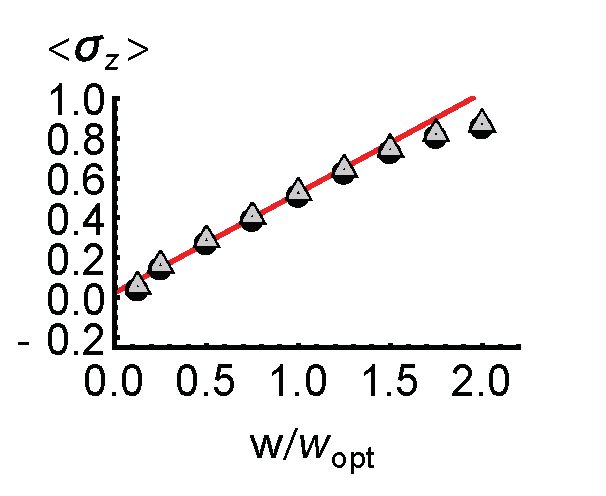
\includegraphics[scale =0.38] {N40SuperradianceSZ.eps}
	\hspace{-5.0mm} 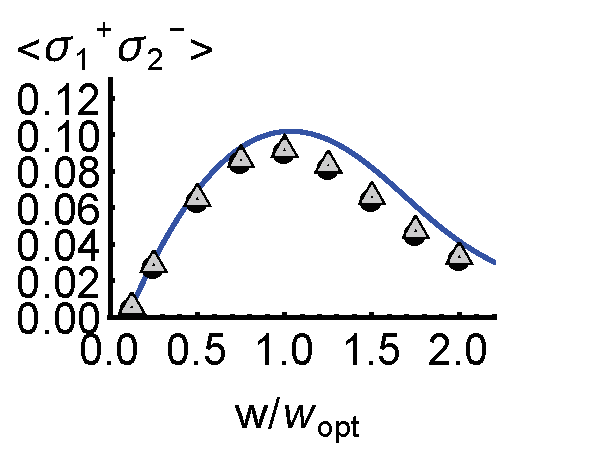
\includegraphics[scale =0.38] {N40SuperradianceSPSM.eps}
	\hspace{-5.0mm} 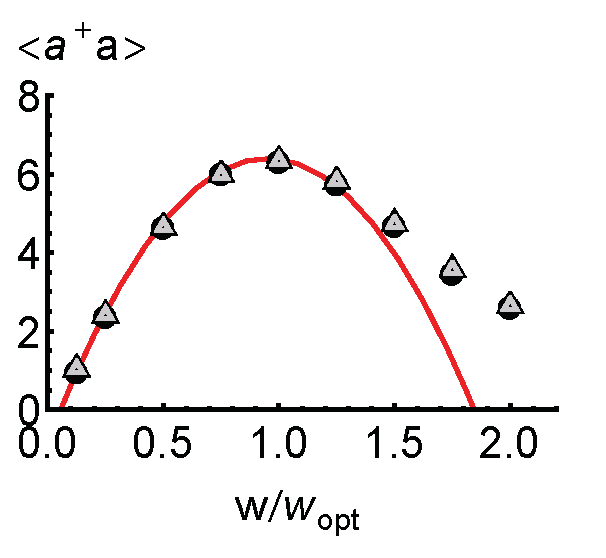
\includegraphics[scale =0.38] {N40Superradianceada.eps}
	\hspace{-5.0mm} 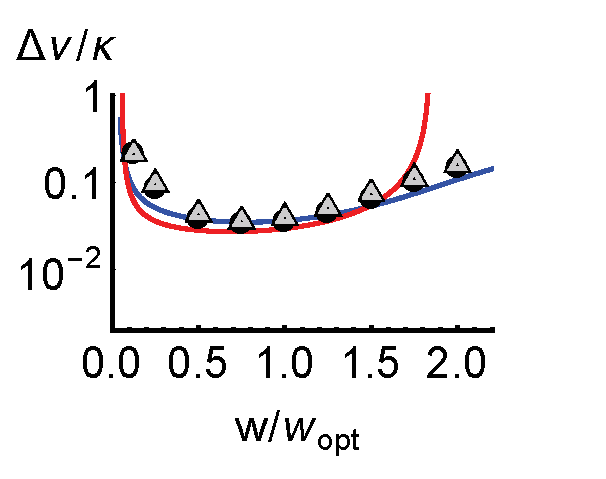
\includegraphics[scale =0.38] {N40SuperradianceLW.eps}
	\hspace{-5.0mm} 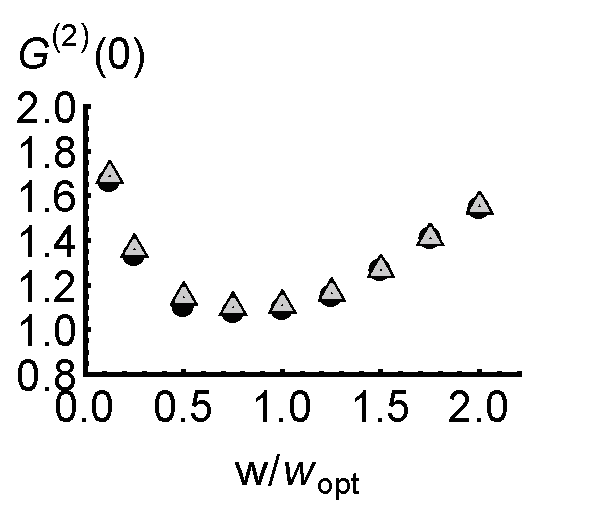
\includegraphics[scale =0.38] {N40SuperradianceG2.eps}\\ \vspace{0mm}
	\rotatebox{90}{ \hspace{7mm} \textbf{Crossover}}
	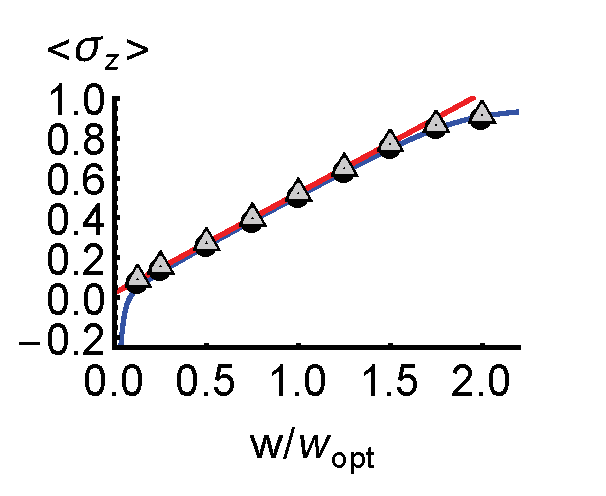
\includegraphics[scale =0.38] {N40CrossoverSZ.eps}
	\hspace{-5.0mm} 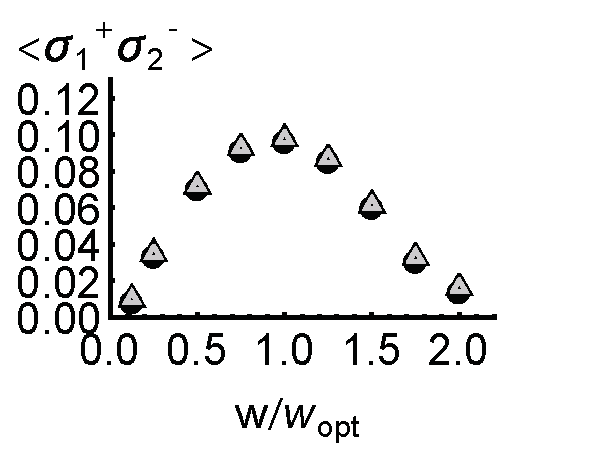
\includegraphics[scale =0.38] {N40CrossoverSPSM.eps}
	\hspace{-5.0mm} 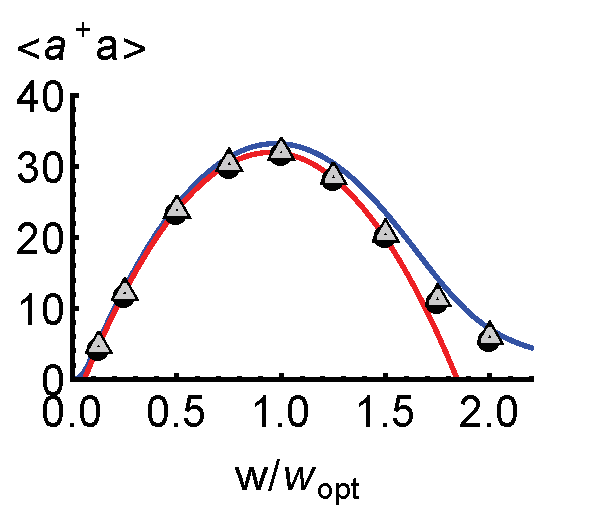
\includegraphics[scale =0.38] {N40Crossoverada.eps}
	\hspace{-5.0mm} 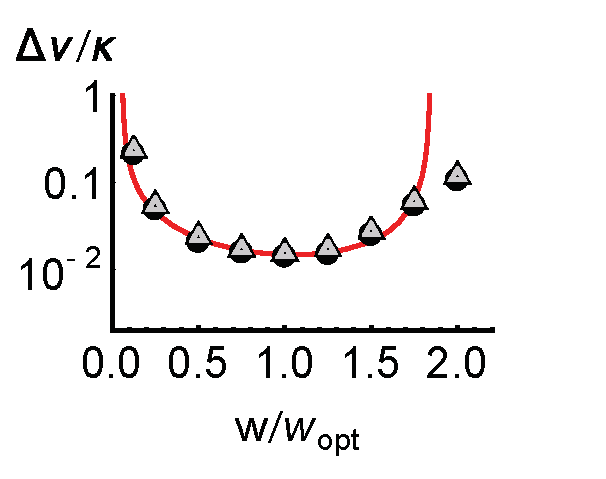
\includegraphics[scale =0.38] {N40CrossoverLW.eps}
	\hspace{-5.0mm} 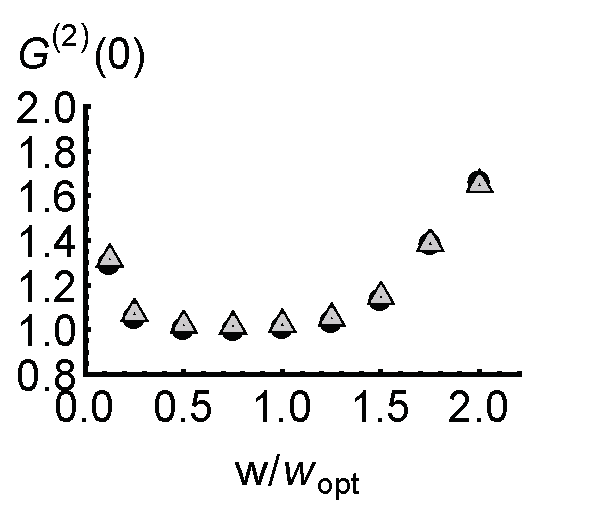
\includegraphics[scale =0.38] {N40CrossoverG2.eps}\\ \vspace{0mm}
	\rotatebox{90}{ \hspace{10mm} \textbf{Lasing}}
	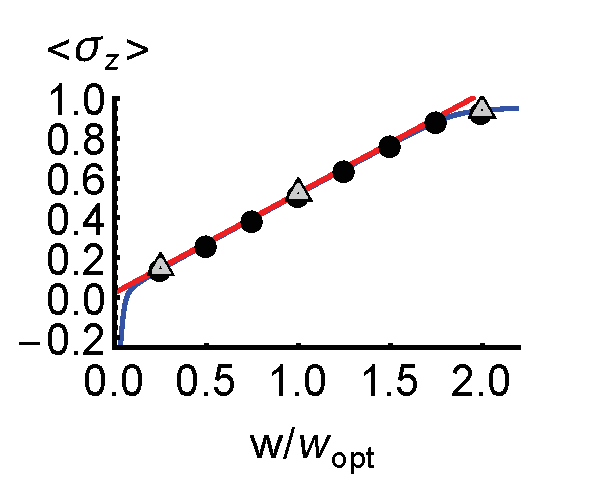
\includegraphics[scale =0.38] {N40LaserSZ.eps}
	\hspace{-5.0mm} 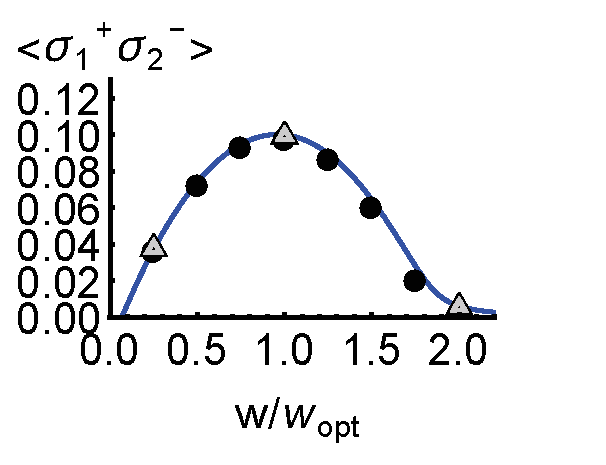
\includegraphics[scale =0.38] {N40LaserSPSM.eps}
	\hspace{-5.0mm} 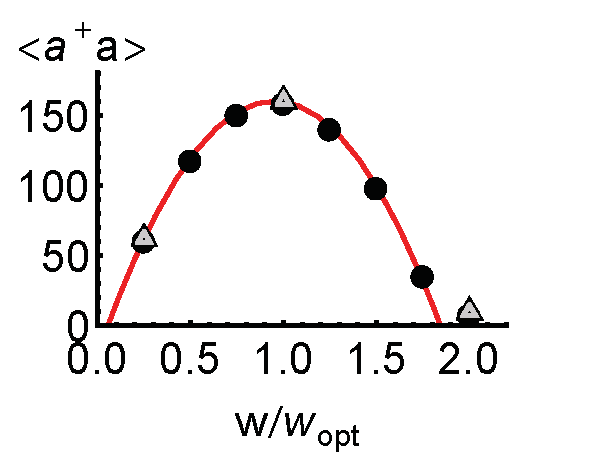
\includegraphics[scale =0.38] {N40Laserada.eps}
	\hspace{-5.0mm} 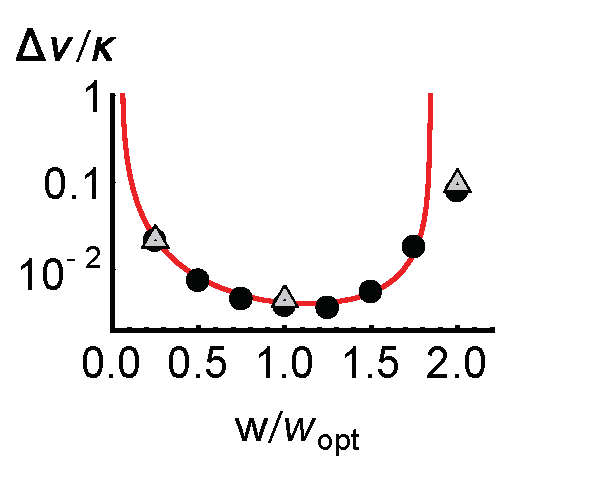
\includegraphics[scale =0.38] {N40LaserLW.eps}
	\hspace{-5.0mm} 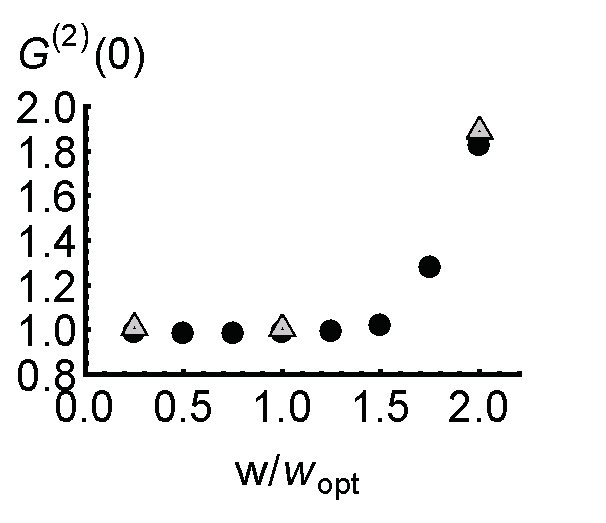
\includegraphics[scale =0.38] {N40LaserG2.eps}\\ \vspace{1mm}
	\hspace{5mm}(a)\hspace{30mm}(b) \hspace{30mm}(c) \hspace{30mm}(d) \hspace{30mm}(e)
\end{center}
		\vspace{-5mm}
\caption{(Color online) Comparison of the different solution methods in
the superradiance ($\xi=0.2$), crossover ($\xi=1$), and lasing ($\xi=5$)
regions for $N=40$ and $\frac{\Omega^2}{\kappa \gamma}=1$.  The analytic
Langevin (phase diffusion and mean field) solutions are shown in red
(light gray), the exact SU(4) solution is shown by grey triangles, and the {\it
c}-number Langevin simulation results are shown by black circles. The
observables considered are (a) the inversion
$\left<\hat{\sigma}^{z}\right>$, (b) the correlation between the atoms'
dipoles $\left<\hat{\sigma}_{1}^{+} \hat{\sigma}_{2}^{-}\right>$, (c)
the intracavity photon number  $\left<\hat{a}^{\dagger}\hat{a}\right>$,
(d) the linewidth $\Delta \nu$, and (e) the intensity correlation
function $G^{(2)}(0)$.}
\label{N40Comparison}
\end{figure*}


\section{Characterization of the Crossover}
\label{sec:CrossoverCharacterization}

\dmcomment{This section is still kind of weak.  Why should I think of
Eqn (\ref{CrossoverParameter}) as the crossover parameter?  Is the
reasoning backwards?  Perhaps we should start from $\xi=a_0^2/N$?  $\xi$
just doesn't seem well motivated the way it's presented here. DT Answer: Im happy to reverse the motivation if it more clear that way.}

The mean field equations allow us to formulate and discuss one of the
central results of this paper, a characterization of the crossover from
lasing to superradiance.  One way to look at the crossover is as the
transition from a good cavity to a bad cavity system.  This suggests the
crossover parameter $\xi$ to be the ratio of the maximum atomic decay
rate (including repumping $w$ and dephasing $1/T_2$) to the cavity
linewidth $\kappa$,
\begin{equation}
\xi\equiv\frac{ w_{opt}+\gamma+\frac{1}{T_2}}{4\kappa}.
\label{CrossoverParameter}
\end{equation}
We can write $\xi$ more concisely by inserting Eq.~(\ref{wopt}),
\begin{equation}
\xi\equiv \frac{N \Omega^2}{8\kappa^2}\;.
\label{CrossoverParameter2}
\end{equation}
In this form it is apparent that $\xi$ is given by the ratio of the
collective atomic decay rate to the cavity decay rate.  This
interpretation can be made more explicit by inserting the maximum photon
number to write
\begin{equation}
\xi = \frac{(|a_0|^2)_{opt}}{N},
\end{equation}
The dimensionless parameter $\xi$ quantifies the relative importance of
stimulated emission to collective atomic effects. If $\xi\ll1$, the
system is in the bad cavity or superradiant regime. If $\xi\gg1$ the
system is in the good cavity or laser regime. The region $\xi\sim1$
defines the intermediate or crossover regime.


\section{Results}
\label{sec:Results}

In this section we present numerical results for field intensity,
inversion, line widths, and correlations throughout the crossover from
lasing to superradiance.  We begin by considering the different solution
methods for small numbers of atoms were we can compare with the exact
SU(4) Monte-Carlo results.  This comparison shows that the semi-classical
theory gives an accurate description of first and second moments of the
system operators.  This is an interesting result in itself besides
verifying the semi-classical methods because it demonstrates that the
system is not strongly correlated and we don't need to account for
genuinely quantum fluctuations.

With the validity of the semi-classical method established we then
consider systems with large numbers of atoms.  These systems are
experimentally relevant and allow us to more clearly understand the
behavior of the system in the large $N$ limit.

\begin{figure*}
\begin{center}
	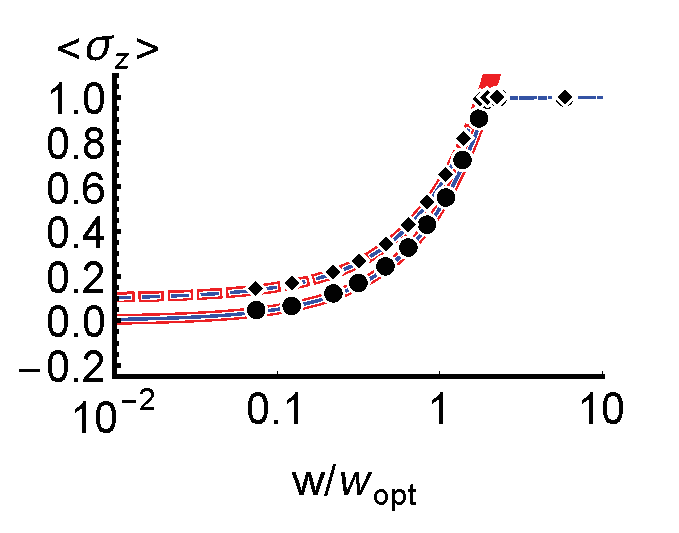
\includegraphics[scale =0.445] {N10000SZ.eps}
	\hspace{-5.0mm} 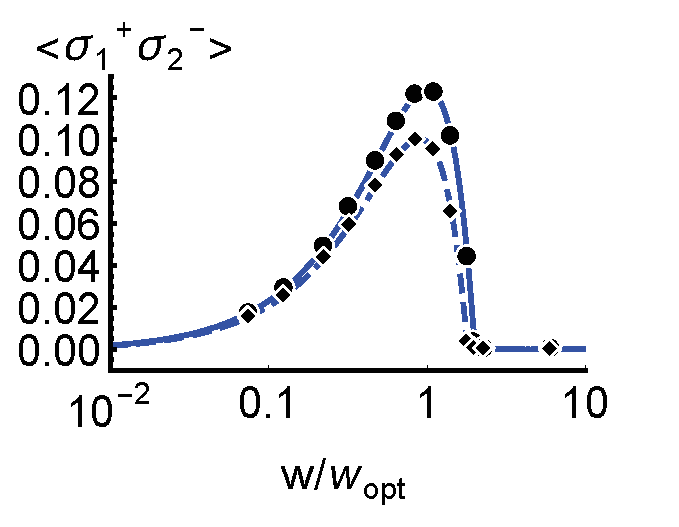
\includegraphics[scale =0.445] {N10000SPSM.eps}
	\hspace{-6.5mm} 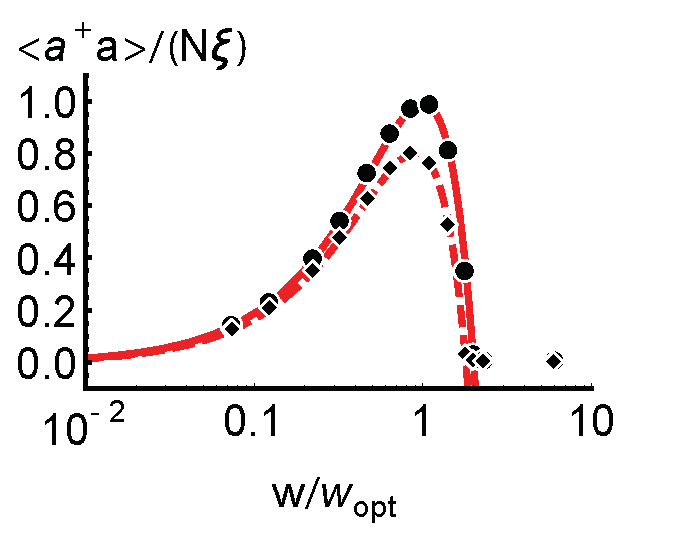
\includegraphics[scale =0.445] {N10000ada.eps}
	\hspace{-5.5mm} 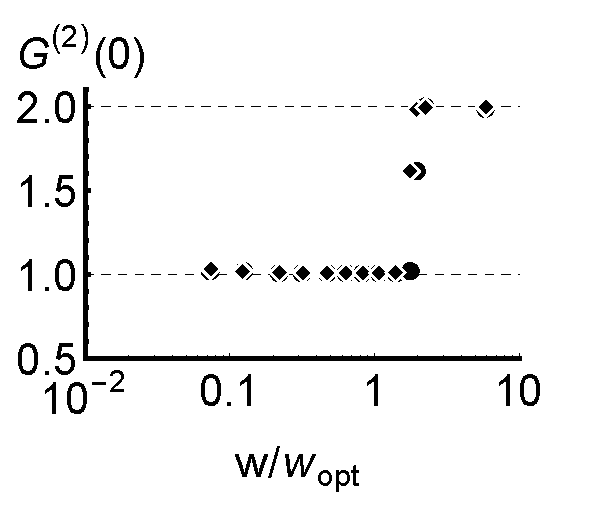
\includegraphics[scale =0.445] {N10000G2S.eps}\\
	\textbf{(a) Universal}\\
	\line(1,0){500}\\
	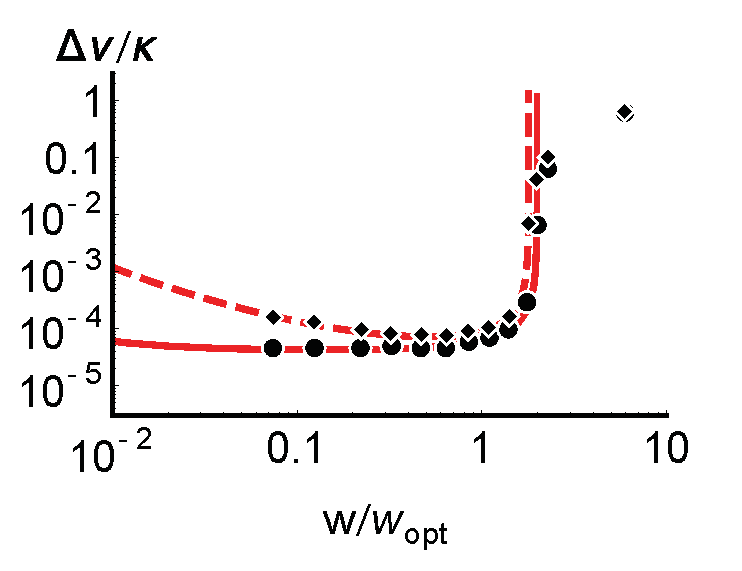
\includegraphics[scale =0.51] {N10000LWS.eps}
	\hspace{-5.5mm} 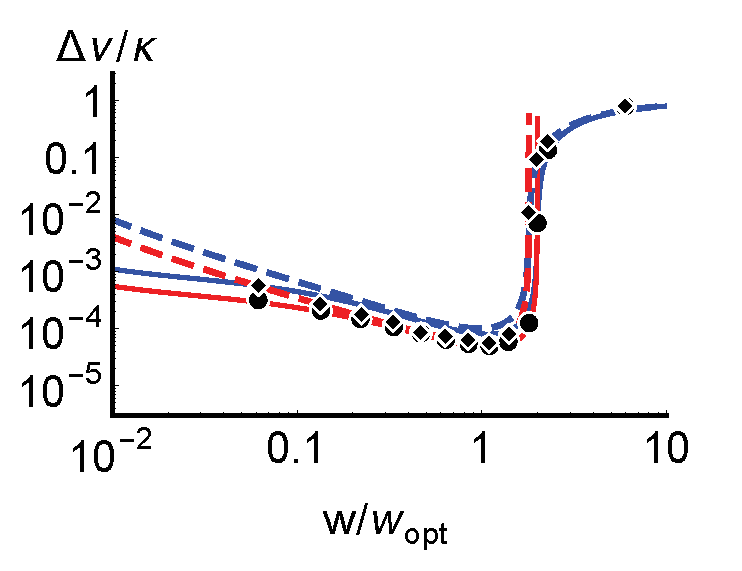
\includegraphics[scale =0.51] {N10000LWC.eps}
	\hspace{-5.5mm} 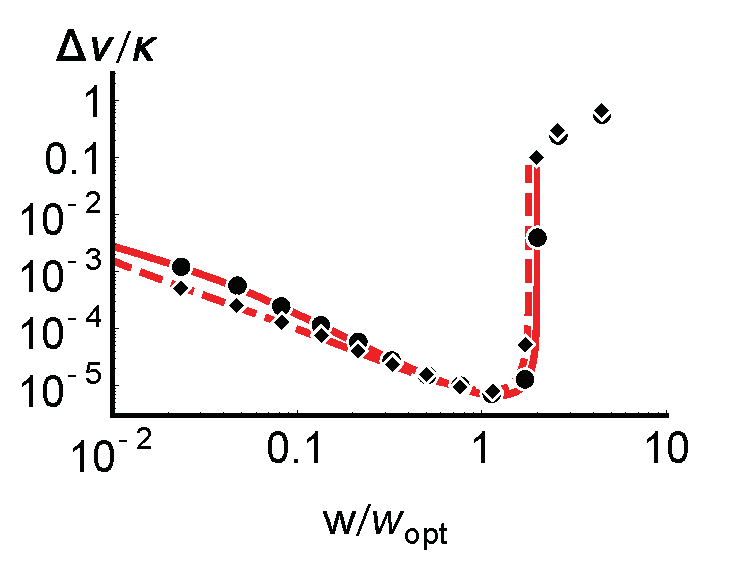
\includegraphics[scale =0.51] {N10000LWL.eps}\\
	\hspace{-10mm}\textbf{(b) Superradiance}\hspace{33mm}\textbf{(c) Crossover}
  \hspace{37mm}\textbf{(d) Lasing}
\end{center}
		\vspace{-5mm}
\caption{(Color online) Solutions using the various methods in the
superradiance ($\xi=0.1$), crossover ($\xi=1$), and lasing ($\xi=10$)
regions for N=10000 and $\frac{\Omega^2}{\kappa \gamma}=0.1$. For
$1/T_2=0$, the analytic Langevin (phase diffusion and mean field)
solutions are shown in solid red (solid light gray), and the
{\it c}-number Langevin simulation results are shown by black circles.
For $1/T_2=\frac{1}{5} w_{opt}$, the analytic Langevin solutions are
shown in dashed red (dashed light gray), and the {\it
c}-number Langevin simulation results are shown by black diamonds. (a)
All observables considered except linewidth  $\Delta \nu$ show universal
behavior in the superradiance, crossover, and lasing regions, after
appropriate scaling.  (b)  $\Delta \nu / \kappa$ in the superradiance
region (c) $\Delta \nu / \kappa$ in the crossover region, (d) $\Delta
\nu / \kappa$ in the lasing region.}
 \label{N10000Comparison}
\end{figure*}


\subsection{Simulations with small atom numbers}

In order to determine the validity of the approximate solution methods,
we begin by comparing them to the exact solutions.  We use $N=40$ atoms
for the comparison.  This is a small enough to still be tractable by
exact SU(4) Monte-Carlo simulations and at the same time it is large
enough to expect the approximate solution methods to be reasonably
accurate. 

Specifically, Fig.~\ref{N40Comparison} shows several observables
obtained using the mean field Langevin method, the phase diffusion
method, the {\it c}-number Langevin method, and exact SU(4) Monte-Carlo
simulations for three different values of the crossover parameter:
$\xi=0.2$, $\xi=1$, and $\xi=5$. These values of $\xi$ put the system in
the superradiance, crossover, and lasing parameter regions,
respectively.  We note that the SU(4) method becomes more
computationally intensive as $\xi$ is increased, since there are more
photons as $\xi$ is increased, and hence more basis states need to be
tracked. Therefore, for $\xi=5$, we used a method that combines the
SU(4) approach with the quantum jump method,
see~\cite{PhysRevA.87.062101} for details.

Fig.~\ref{N40Comparison} shows excellent agreement between {\it
c}-number Langevin and the exact SU(4) theory in all parameter regions
for all of the considered observables. Therefore, the {\it c}-number
Langevin theory can be relied upon for larger atom numbers inaccessible
to direct numerical simulation.

Figures~\ref{N40Comparison} (a) and (c) show that the mean field
equations are accurate near the collective emission peak, $w/w_{opt}=1$,
but they are less accurate outside that region.
Figure~\ref{N40Comparison} (d), shows that the phase diffusion model for
the linewidth also agrees in the region around $w/w_{opt}=1$, but
disagrees outside that region, where the phase diffusion approximation
breaks down.  Although they do not quantitatively agree with the exact
SU(4) method, the analytic solutions obtained by the mean field and
phase diffusion models capture the correct qualitative behavior of the
system.


\subsection{Simulations with large atom numbers}

Now that an agreement between the {\it c}-number Langevin and exact
SU(4) theories has been established, we study more experimentally
realistic systems with $N=10000$ using the semi-classical theory based
on the {\it c}-number Langevin equations. We also include the mean field
Langevin theory, the phase diffusion model for the linewidth. The
results of these simulations are shown in Fig.~\ref{N10000Comparison}.
We consider both the case of vanishing inhomogeneous broadening,
$1/T_2=0$, as well as $1/T_2=w_{opt}/5$.

As seen in Fig.~\ref{N10000Comparison} (a), when $1/T_2=0$, the
inversion $\left<\hat{\sigma}^{z}\right>$, the correlation between atoms
$\left<\hat{\sigma}_{1}^{+} \hat{\sigma}_{2}^{-}\right>$, the
intracavity photon number  $\left<\hat{a}^{\dagger}\hat{a}\right>$,  and
the intensity correlation function $G^{(2)}(0)$ all show universal
behavior in the superradiance, crossover, and lasing regimes after
appropriate scaling.  For $1/T_2=w_{opt}/5$ these observables still show
universal behavior after appropriate scaling, and the values do not
change significantly from the $1/T_2=0$ case.

It is worth noting that, even though  $\left<\hat{\sigma}_{1}^{+}
\hat{\sigma}_{2}^{-}\right>$ has universal behavior throughout the
crossover, typical lasers operate just above threshold in terms of the
scaled quantities, i.e. $w \ll w_{opt}$.  Just above threshold the
atom-atom correlations are typically very small,
\begin{equation}
\left<\hat{\sigma}_{1}^{+}\hat{\sigma}_{2}^{-}\right>_{opt} \ll 1\;.
\end{equation}
Thus atom-atom correlations are usually not important in lasers.

The linewidth $\Delta \nu$, however, does not show universal behavior in
the superradiance, crossover, and lasing regimes. As seen in
Fig.~\ref{N10000Comparison} (b), in the superradiance region, when
$1/T_2=0$, $\Delta \nu / \kappa$ is flat in the region of $w/w_{opt}<1$.
In contrast, the linewidth in the lasing regime, shown in
Fig.\ref{N10000Comparison} (d), linearly decreases as $w/w_{opt}$
increases towards unity. This is the typical Schawlow-Townes behavior,
which can be seen by considering
$\kappa/\left<\hat{a}^{\dagger}\hat{a}\right>$ using Eq.~\ref{a0sqSS}.
In the crossover region, shown in Fig.~\ref{N10000Comparison} (c), we
see that for $w/w_{opt}\ll 1$ , $\Delta \nu/\kappa$ is flat, and as
$w/w_{opt}$ approaches unity, $\Delta \nu/\kappa$ starts to linearly
decrease as in the lasing regime. Therefore, a system in the crossover
region displays characteristics of both superradiance and lasing. 

When $1/T_2$ is increased to $1/T_2=w_{opt}/5$,
Fig.~\ref{N10000Comparison} (b) shows that $\Delta \nu/\kappa$ increases
for $w/w_{opt}\ll 1$, but it is not significantly affected by $1/T_2$ as
$w/w_{opt}$ approaches unity.  Note that the latter is the pumping
region where the emitted light intensity is largest.  Near $w\sim w_{\rm
opt}$ we obtain both the largest intensity and the best frequency
stability.

In the crossover region, seen in Fig.~\ref{N10000Comparison} (c), when
$1/T_2=w_{opt}/5$, $\Delta \nu/\kappa$ increase for $w/w_{opt}\ll 1$,
where the system is displaying superradiant behavior.  On the other
hand, when $w \sim w_{opt}$ where the
system starts to display lasing behavior, $\Delta\nu/\kappa$ is
insensitive to the inhomogeneous broadening of the atomic line.
\begin{figure}
\begin{center}
	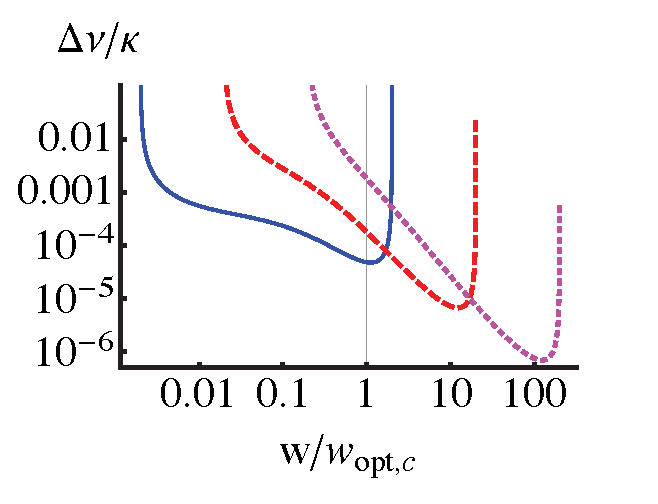
\includegraphics[scale =0.415] {LinewidthComparisonLangevin.eps}
	\hspace{-4mm} 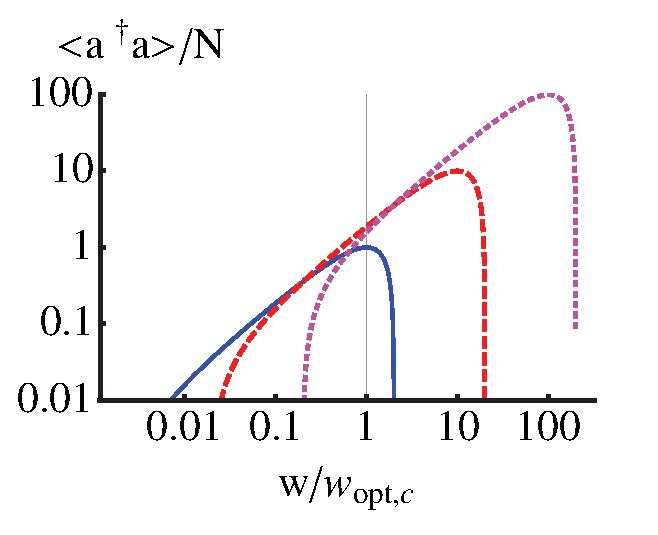
\includegraphics[scale =0.415] {adaComparisonLangevin.eps}\\
	\hspace{6mm}\textbf{(a)}\hspace{37mm}\textbf{(b)} \hspace{35mm}
\end{center}
		\vspace{-5mm}
\caption{(Color online) Comparison of (a) linewidth and (b) intra-cavity
intensity for a system in the crossover ($\xi=1$) shown in blue solid,
lasing ($\xi=10$) shown in red dashed, and far lasing ($\xi=100$) shown
in magenta dotted, regions using the analytic (phase diffusion and mean
field) Langevin model. $w_{opt,c}$ is the optimum $w$ value in the
crossover region. For all systems, $N=10000$ and $\frac{\Omega^2}{\kappa
\gamma}=0.1$.}
\label{LWadaComparison}
\end{figure}

Figure~\ref{N10000Comparison} (d) shows that $\Delta \nu/\kappa$ does
not increase in the lasing region when $1/T_2=w_{opt}/5$.  Rather the
linewidth decrease in the region slightly below $w/w_{opt}=1$, when
compared to the $1/T_2=0$ case. This reduction has also been observed
for smaller atom numbers using the exact SU(4) code. It can be shown
that the value of $1/T_2$ that maximally reduces the linewidth is
$1/T_2=\frac{w_{opt}}{1+\sqrt{2}}$.
\dmcomment{Do we have an intuitive explanation of this result? DT Answer: I do not have an intuitive understanding of this result. I included it just incase it sparked the interest of someone else.}

As mentioned previous, a laser normally operates just above threshold,
where $w/w_{opt} \ll 1$. As seen in Fig.~\ref{LWadaComparison} (a), for
the same pump strength $w$, and a fixed $N$, a system in the crossover
region can operate with $w/w_{opt} = 1$, allowing the crossover system
to have a linewidth orders of magnitude smaller than the linewidth of
the lasing system.  Fig.~\ref{LWadaComparison} (b) shows that this
improvement in linewidth can be achieved without paying the penalty of a
reduced output intensity.  Another way of saying this is that, for the
same output intensity, one can achieve greater brightness of the light
source by using atoms with a smaller linewidth.


\subsection{Robustness against level shifts}

The sensitivity to systematic level shifts is another key figure of
merit of this light source, especially in the context of precision
measurements and for applications as a local oscillator.  The intrinsic
linewidth discussed so far assumes a perfectly stable cavity and atomic
resonance frequency.  However, in real world systems these resonance
frequencies are subject to temporal variations.  For example, thermal
fluctuations of the dielectric coatings of the cavity mirrors cause
fluctuations of the cavity resonance frequency.  Stray electric and
magnetic fields cause atomic level shifts.  An important special case of
the latter are black body shifts.
\begin{figure}
\begin{center}
	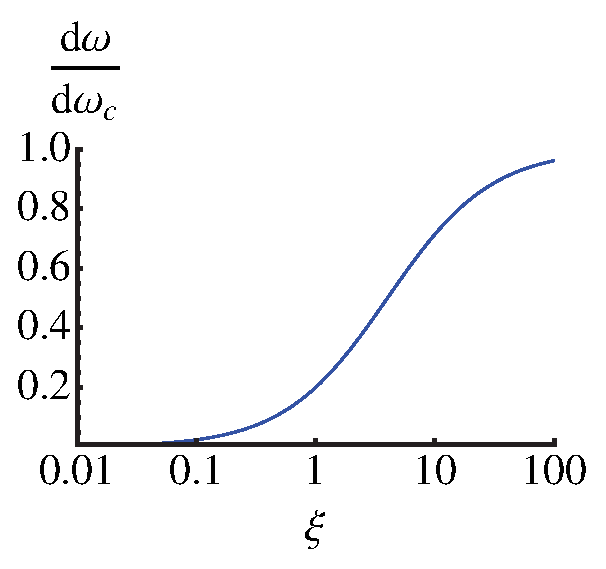
\includegraphics[scale=0.42] {CavityInstability.eps} \hspace{2mm}
	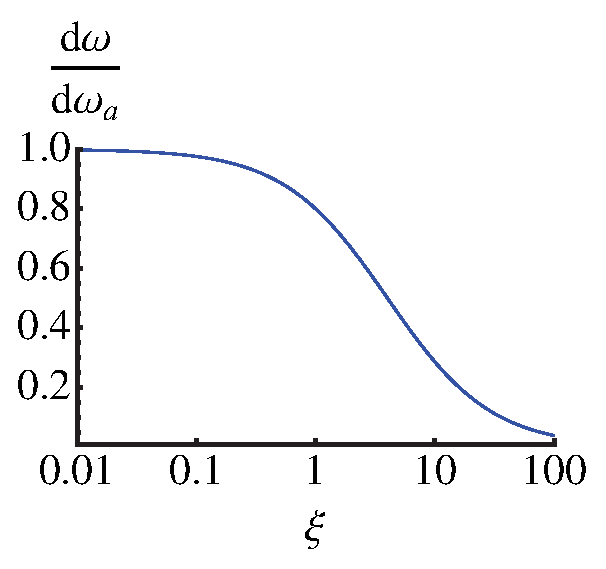
\includegraphics[scale=0.42] {AtomInstability.eps}\\
\hspace{2mm} \textbf{(a)}\hspace{40mm}\textbf{(b)} \hspace{35mm}
\end{center}
\caption{(Color online) Instability in the atom-cavity system frequency
$\omega$ with respect to (a) the cavity frequency $\omega_c$ and (b)
atomic frequency $\omega_a$ as a function of the crossover parameter
$\xi$.}
\label{CavityInstability}
\end{figure}

In the limit where the atomic and cavity frequencies vary slowly
\dmcomment{Compared to what? Is this the important limit? What is the
spectrum of the fluctuations?} we find the sensitivity of the coupled
atom-cavity system from Eq.~(\ref{atomcavityfrequencycenter1}).  The
derivatives of the emission frequency with respect to $\omega_c$ and
$\omega_a$ is shown in Fig.~\ref{CavityInstability}.  On the
superradiance side of the crossover, $\xi \ll 1$, the system is
sensitive to fluctuations of the atomic resonance frequency but
sensitivity to fluctuations of the cavity resonance frequency is
suppressed by a factor $\xi$.  On the lasers side of the resonance the
situation is reversed.  The steady state superradiance regime thus holds
promise for the development of light sources that overcome the $1/f$
noise due to thermal fluctuations in the mirror substrates.


\section{Conclusion}

In this paper we have theoretically studied the continuous crossover
from steady state superradiance to lasing.  We have developed a
semi-classical approximation based on $c$-number Langevin equations and
we have verified the accuracy of this model by comparison with a direct
numerical solution of the open quantum system dynamics using quantum
Monte-Carlo simulations.  We have introduced a dimensionless parameter
that characterizes the crossover.  One interpretation of the crossover
parameter is as the ratio of the intracavity photon and atom numbers or,
equivalently, the relative importance of stimulated emission and
collective interference, respectively.

We have systematically investigated the generated intensity, the
linewidth of the light source, intensity correlations, and the
sensitivity to systematic perturbations of the cavity resonance
frequency and the atomic transition frequency.  We find that, for a given
output intensity, the system has a smaller intrinsic linewidth and is
less sensitive to cavity pulling by operating closer to the
superradiance  regime.

Throughout the crossover the system is insensitive to atomic dephasing
provided that the re-pumping rate is larger than the dephasing rate.
Surprisingly, on the laser side, atomic dephasing can even lead to a
reduction of the linewidth of the emitted light.

This work has been supported by JILA-NSF-PFC-1125844, DARPA, QuASAR, and
NIST.

\appendix


\section{Phase Diffusion Linewidth}
\label{HakenAppendix}

In this appendix we derive a closed form expression for the linewidth
based on a phase diffusion model.  Our analysis closely follows the
derivation in~\cite{HakenLaser, HakenLaserBook}.

Differentiating Eq.~(\ref{La}) with respect to time and substituting 
Eqns.~(\ref{La})~--~(\ref{Lsm}) we obtain
\begin{equation}
\ddot{\hat{a}} =
-\frac{1}{2} (\kappa+\Gamma)  \dot{\hat{a}} -
\frac{\kappa \Gamma}{4}\hat{a}  +
\frac{N \Omega^2 }{4} \hat{a} \hat{S}^z +\hat{F},
\label{addeq}
\end{equation}
where
\begin{eqnarray}
\hat{S}^z &=&
\int_0^t dt^{\prime} e^{-(w+\gamma)(t-t^{\prime})}
\bigg( (w+\gamma) + \hat{F}^z
\nonumber
\\
&&\hspace{-3mm}-\frac{2}{N} \left( \frac{d}{dt} (\hat{a}^{\dagger} \hat{a}) +
\kappa \hat{a}^{\dagger} \hat{a} -\hat{a}^{\dagger} \hat{F}^a -
\hat{F}^{a^{\dagger}} \hat{a} \right) \bigg),
\end{eqnarray}
and
\begin{equation}
\hat{F} = \frac{\Gamma}{2} \hat{F}^a-
\frac{i N \Omega}{2} \hat{F}^-+\dot{\hat{F}}^a.
\end{equation}

The annihilation operator $\hat{a}$ is decomposed according to,
\begin{equation}
\hat{a}= (a_0 + \hat{\rho}) e^{i\hat{\phi}}.
\label{adecomp}
\end{equation}
Above threshold, amplitude fluctuations are small so that $\hat\rho$
can be neglected.  We then obtain for the two time correlation function
of the field amplitude
\begin{equation}
\left< \hat{a}^{\dagger}(t) \hat{a}(0) \right> =
a_0^2 \left< e^{i(\hat{\phi}(t) - \hat{\phi}(0))} \right>.
\end{equation}

After substituting Eq.~(\ref{adecomp}) into Eq.~(\ref{addeq}), we take
the imaginary part to first order in products of operators, and find,
\begin{equation}
\ddot{\hat{\phi}} =
-\frac{1}{2}(\kappa+\Gamma) \dot{\hat{\phi}} +
\frac{1}{a_0} \text{Im} [\hat{F}],
\label{phieq1}
\end{equation}
where a factor of $e^{-i\phi}$ has been absorbed into $\hat{F}$.
Eq.~(\ref{phieq1}) is then integrated, assuming that $(\kappa+\Gamma)$
is large, to arrive at,
\begin{equation}
\hat{\phi}(t) - \hat{\phi}(0) =
\frac{2}{a_0 (\kappa+\Gamma)}
\int_0^t dt^{\prime} \text{Im}
\left[ \frac{\Gamma}{2} \hat{F}^a-\frac{i N \Omega}{2} \hat{F}^-\right]\;.
\label{phieq2}
\end{equation}
Since $ \hat{F}^a$ and $\hat{F}^-$ are Gaussian, we can use
\begin{equation}
\left< e^{i(\hat{\phi}(t) - \hat{\phi}(0))} \right> =
e^{-\frac{1}{2}\left< ( \hat{\phi}(t) - \hat{\phi}(0) )^2 \right>}.
\end{equation}
Therefore, we use Eq.~(\ref{phieq2}), along with Eqns.~(\ref{OpNoise1})
to find,
\begin{equation}
\left<(\hat{\phi}(t) - \hat{\phi}(0))^2 \right> =
\left(\frac{(C+1)}{2(Cd_0-1)} \frac{\Gamma}{(w+\gamma)}
\frac{\Omega^2 \kappa}{(\kappa+\Gamma)^2}\right) t,
\end{equation}
so that the linewidth $\Delta \nu$ given by,
\begin{equation}
\Delta \nu =
\frac{(C+1)}{2(Cd_0-1)} \frac{\Gamma}{(w+\gamma)}
\frac{\Omega^2 \kappa}{(\kappa+\Gamma)^2}.
\label{LWHaken}
\end{equation}

\bibliographystyle{unsrt}
\bibliography{CrossoverPaper}

\end{document}

% vim: nocindent spell
